%% ****** Start of file apstemplate.tex ****** %
%%
%%
%%   This file is part of the APS files in the REVTeX 4 distribution.
%%   Version 4.1 of REVTeX, October 2009
%%
%%
%%   Copyright (c) 2001, 2009 The American Physical Society.
%%
%%   See the REVTeX 4 README file for restrictions and more information.
%%
%
% This is a template for producing manuscripts for use with REVTEX 4.0
% Copy this file to another name and then work on that file.
% That way, you always have this original template file to use.
%
% Group addresses by affiliation; use superscriptaddress for long
% author lists, or if there are many overlapping affiliations.
% For Phys. Rev. appearance, change preprint to twocolumn.
% Choose pra, prb, prc, prd, pre, prl, prstab, prstper, or rmp for journal
%  Add 'draft' option to mark overfull boxes with black boxes
%  Add 'showpacs' option to make PACS codes appear
%  Add 'showkeys' option to make keywords appear
\documentclass[aps,prb,preprint,groupedaddress,amsmath]{revtex4}
%\documentclass[aps,prl,preprint,superscriptaddress]{revtex4-1}
%\documentclass[aps,prl,reprint,groupedaddress]{revtex4-1}

% You should use BibTeX and apsrev.bst for references
% Choosing a journal automatically selects the correct APS
% BibTeX style file (bst file), so only uncomment the line
% below if necessary.
%\bibliographystyle{apsrev4-1}
\usepackage{graphicx}
\newcommand{\vp}{\ensuremath{\mathbf{p}}}
\newcommand{\vk}{\ensuremath{\mathbf{k}}}
\newcommand{\dg}{\ensuremath{\dagger}}

\begin{document}

% Use the \preprint command to place your local institutional report
% number in the upper righthand corner of the title page in preprint mode.
% Multiple \preprint commands are allowed.
% Use the 'preprintnumbers' class option to override journal defaults
% to display numbers if necessary
%\preprint{}

%Title of paper
\title{BCS ansatz, Richardson's exact eigenstate and the Pauli exclusion principle}

% repeat the \author .. \affiliation  etc. as needed
% \email, \thanks, \homepage, \altaffiliation all apply to the current
% author. Explanatory text should go in the []'s, actual e-mail
% address or url should go in the {}'s for \email and \homepage.
% Please use the appropriate macro foreach each type of information

% \affiliation command applies to all authors since the last
% \affiliation command. The \affiliation command should follow the
% other information
% \affiliation can be followed by \email, \homepage, \thanks as well.
\author{}
%\email[]{Your e-mail address}
%\homepage[]{Your web page}
%\thanks{}
%\altaffiliation{}
\affiliation{}

%Collaboration name if desired (requires use of superscriptaddress
%option in \documentclass). \noaffiliation is required (may also be
%used with the \author command).
%\collaboration can be followed by \email, \homepage, \thanks as well.
%\collaboration{}
%\noaffiliation

\date{\today}

\begin{abstract}
% insert abstract here
\end{abstract}

% insert suggested PACS numbers in braces on next line
\pacs{}
% insert suggested keywords - APS authors don't need to do this
%\keywords{}

%\maketitle must follow title, authors, abstract, \pacs, and \keywords
\maketitle

% body of paper here - Use proper section commands
% References should be done using the \cite, \ref, and \label commands
\section{Formalism for composite bosons\label{sec:formalism}}
\subsection{Free pairs}
We consider free pair states with one degree of freedom only, namely
\begin{equation}\label{eq:beta}
\beta_\vk^\dg=a^\dg_{\vk\uparrow}{}a^\dg_{-\vk\downarrow}
\end{equation}
 In BCS superconductivity, these free fermion pairs feel a potential taken as constant and separable in a layer of extension $\Omega$ above a frozen Fermi sea $|F_0{\rangle}$, namely
\begin{equation}
V_{BCS}=-V\sum_{\vk'\vk}w_{\vk'}w_{\vk}\beta^\dg_{\vk'}\beta^{}_\vk
\label{eq:}
\end{equation}
with $w_\vk=1$ for $\epsilon_{F_0}<\epsilon_\vk<\epsilon_{F_0}+\Omega$. The BCS potential thus scatters any $\vk$ pair state of the potential layer into any other $\vk'$ pair state, with the same attractive strength V.

The statistical properties of these free pair states follow from their composite boson nature which results from the Pauli exclusion principle between their fermionic components. It shows up through
\begin{equation}  
\left[\beta^{\dagger}_{\mathbf{k} ^{\prime}},\beta^{\dagger}_{\mathbf{k} }%
\right]  =0
\end{equation}
\begin{equation}  \label{eq:betacom}
\left[\beta_{\mathbf{k} ^{\prime}},\beta^{\dagger}_{\mathbf{k} }\right] 
=\delta_{\mathbf{k} ^{\prime}\mathbf{k} }-\mathit{D} _{\mathbf{k} ^{\prime}%
\mathbf{k} }
\end{equation}
where the "deviation-from-boson operator" $\mathit{D} _{\mathbf{k} ^{\prime}\mathbf{k} }$ is equal to
\begin{equation}\label{eq:D}
\mathit{D} _{\mathbf{k} ^{\prime}\mathbf{k} }=\delta_{\mathbf{k} ^{\prime}\mathbf{k}}\sum_{s=(\uparrow,\downarrow)}a^\dg_{\vk{s}}{}a^{}_{\vk{s}}
\end{equation}
 When acting on another free pair, this operator gives
\begin{equation}
\left[\mathit{D} _{\mathbf{p}\mathbf{k} ^{}_1},\beta^{\dagger}_{%
\mathbf{k} _2}\right]  =2\delta_{\mathbf{k}_1 \mathbf{p} }\delta_{\mathbf{k}_2 \mathbf{p} }\beta_\vp^\dg
\end{equation}

The interaction properties of the $\beta_\vp^\dg$ free pairs follow from commutations with the system hamiltonian $H=H_0+V_{BCS}$, the kinetic part reading as $H_0=\sum_{\vk{s}}\epsilon_\vk{}a^\dg_{\vk{s}}a^{}_{\vk{s}}$. We then find
\begin{equation}  \label{eq:betaH}
\left[H_0,\beta^{\dagger}_\vp\right]  =2\epsilon_\vp\beta^{\dagger}_\vp
\end{equation}
\begin{equation}  \label{eq:vbeta}
\left[V_{BCS},\beta^{\dagger}_\vp\right] 
=-Vw^{}_\vp\beta^{\dagger}+V^{\dagger}_\vp
\end{equation}
where 
\begin{equation}
\beta^{\dagger}=\sum_\vp{}w_\vp\beta^{\dagger}_\vp
\end{equation}
\begin{equation}
V^\dg_\vp=-Vw^{}_\vp\beta^{\dagger}\sum_s{}a^\dg_{\vp{s}}a^{}_{\vp{s}}
\end{equation}
Due to the $w_\vp$ part of the $V^\dg_\vp$ operator, we do have $V^\dg_\vp|F_0{\rangle}=0$ while its action on a $\beta_\vp^\dg$ free pair follows from 
\begin{equation}  \label{eq:vpotbeta}
\left[V^{\dagger}_{\mathbf{p} _2},\beta^{\dagger}_{\mathbf{p} _1}\right] 
=2V\delta_{\mathbf{p} _1\mathbf{p} _2}w_{\mathbf{p} _1}\beta^{\dagger}_{\mathbf{p} _1}\beta^{\dagger}_{}
\end{equation}

\subsection{Correlated pairs}

%It is actually quite easy to write the recursive relation fulfilled by the $f_N$'s.  For that let us introduce the operator

We now consider correlated pairs, i.e., linear combination of free pairs. Due to the form of the BCS potential which scatters any pair state belonging to the potential layer into any other pair state, the linear combination of free pairs relevant in BCS superconductivity must a priori contain all the pairs feeling the potential layer.

 It also is of importance to note that, unlike excitons, the correlated pairs which are going to be of interest in BCS superconductivity are not the one-pair eigenstates of the system. As a direct consequence, they do not form a complete basis in the one-pair subspace, so that we cannot go back and forth from free to correlated pairs as we did in the case of excitons. This makes the handling of many-body effects between BCS pairs far more complicated than between excitons. 

To possibly derive many-body effects between BCS pairs in a compact way, it is actually necessary to introduce their generalized form defined as 
\begin{equation}\label{eq:C}
{C}_m^\dg=\sum{w_\vk\varphi_\vk|\varphi_\vk|}^{2m}\beta^\dg_\vk
\end{equation}
these correlated pairs being normalized through
\begin{equation}\label{eq:cNormal}
\langle{}F_0|{C_0}{C_0^\dg}|F_0{\rangle}=\sum{w_\vk}|\varphi_\vk|^{2}=1
\end{equation}
The commutators between free pairs introduced above lead to  
\begin{equation}\label{eq:ID}
[{C}_{m'},C^\dg_m]=I_{1+m+m'}-D_{m'm}
\end{equation}
\begin{equation}
[{D}_{m'_1,m_1},C^\dg_{m_2}]=2C^\dg_{1+m_1+m'_1+m_2}
\end{equation}
\begin{equation}
I_m=\sum{w_\vk|\varphi_\vk|^{2m}}
\end{equation}
with $I_1=1$ due to eq. (\ref{eq:cNormal}). The above equations show that, starting with cobosons $C^\dg_0$, we produce a coboson  $C^\dg_1$ after one set of commutations, i.e., one fermion exchange, so that many-body effects induced by fermion exchanges bring $N$ correlated pairs $C^\dg_0$ out of the  ${C^\dg_0}^N$ subspace.

  To derive correlation effects induced by Pauli blocking between $N$ pairs, it is actually convenient to extend the above commutation relations to $N$ correlated pairs. This is easily done by recursion. Eqs. 15 and 14 respectively transform into
\begin{equation}
[{D}_{m0},C^\dg_{0}{}^N]=2N{C^\dg_{0}}^{N-1}C^\dg_{m+1}
\end{equation}
\begin{equation}
[{C}_{m},C^\dg_{0}{}^N]=N{C^\dg_0}^{(N-1)}(I_{1+m}-D_{n0})-N(N-1)C^\dg_{m+1}{C^\dg_{0}}^{N-2}
\end{equation}
As expected, they reduce to Eqs. 15 and 14 for $N=1$.

\subsection{Pauli blocking between $N$ correlated pairs}

These $N$-commutators are necessary to calculate an important quantity to control Pauli blocking between $N$ correlated pairs, namely the normalization factor $f_N$ defined as
\begin{equation}\label{eq:cn}
\langle{}F_0|{C_0^{ }}{}^N{C_0^\dg}{}^N|F_0{\rangle}=N!f_N
\end{equation}
If $C^\dg_0$ were the creation operator of an elementary boson, i.e., for $[C_0,C^\dg_0]$ reducing to 1,  $f_N$ would be equal to 1 for all $N$.  The fact that $f_N$ factor differ from $1$ actually is the signature of "the moth-eaten effect" between composite bosons induced by the Pauli exclusion principle: Each added correlated pair feels the $N$ pairs already present in the system as if $N$ little moths had already eaten $N$ free pair states, taken aleatorily within the $C^\dg_{0}$ sum.  As a result of this effect, $f_N$ is a decreasing function of $N$. 

A direct way to show this decrease is through  the recursion relation fulfilled by the $f_N$'s.  Since $D_{m'm}|F_0\rangle=0 $  as readily seen from Eq. (\ref{eq:ID}) acting on $|F_0\rangle$, the above $N$-commutators give,  as $I_1=1$ 
\begin{equation}
\begin{split} 
\langle{}F_0|{C_0^{ }}{}^N{C_0^\dg}{}^N|F_0{\rangle}&
	=\langle{}F_0|{C_0^{ }}{}^{N-1}[C_0,{C_0^\dg}{}^N]|F_0{\rangle}\\
	&=N\langle{}F_0|{C_0^{ }}{}^{N-1}{C_0^\dg}{}^{N-1}|F_0{\rangle}
	-N(N-1)\langle{}F_0|{C_0^{ }}{}^{N-1}C_1^\dg{C_0^\dg}{}^{N-1}|F_0{\rangle}\\
\end{split}
\end{equation}
To calculate the second term, we  use $[C_0^{N-1},C_1^\dg]$ with $\langle{}F_0|C^\dg_1=0$ due to the $w_\vk$ factor included in $C^\dg_1$. By repeating the process, we end with the following recursion relation between the $f_N$'s 
\begin{equation}\label{eq:fn}
f_N=f_{N-1}-(N-1)I_2f_{N-2}+(N-1)(N-2)I_3f_{N-3}-\cdots+(-1)^{N-1}N!I_Nf_0
\end{equation}
Since $f_0=f_1=1$, we find $f_2=1-I_2,f_3=1-3I_2+2I_3$ and so on... The $f_N$ decrease results from the fact that  the constant $I_N$ defined in Eq.(16) decreases with $N$. This follows from  $|\varphi_\vk|^2$ normalized by  Eq. (\ref{eq:cNormal}) which implies $|\varphi_\vk|^2<1$.

The above recursion relation is convenient to calculate $f_N$ when the RHS is dominated by its first terms, i.e., when the prefactors $N^pI_{p+1}$ are small.  This happens for excitons,  and more generally for correlated pairs in the dilute limit.  In the dense limit however, when Pauli blocking becomes dramatic, the compact form of  $f_N$   given by 
\begin{equation}\label{eq:fn2}
\begin{split}
f_N=\left.\frac{\partial^NZ(x)}{\partial{x^N}}\right|_{x=0}\\
Z(x)=\prod_\vk(1+xw_\vk|\varphi_\vk|^2)
\end{split}
\end{equation}
turns out to be far more convenient. It in particular readily shows that $f_N$ reduces to zero when $N$ gets larger than the number of $\vk$ states having a nonzero $\varphi_\vk$. 

It is possible to check that the above $f_N$ fulfills the recursion relation Eq.(\ref{eq:fn}). Indeed, if $N^*$ is the number of $\vk$ states in the composite boson $C_0^\dg$, the function $Z(x)$
\begin{equation}
%\begin{split}
Z(x)=(1+xw_{\vk_1}|\varphi_{\vk_1}|^2)(1+xw_{\vk_2}|\varphi_{\vk_2}|^2)...(1+xw_{\vk_{N^*}}|\varphi_{\vk_{N^*}}|^2)\\
%=\sum_{N=0}^{N^*}x^Nz_N
%\end{split}
\end{equation}
can be rewritten as
\begin{equation}\label{eq:fz}
Z(x)= \sum_{N=0}^{N^*}x^Nz_N
\end{equation}
where $z_N$ is a sum of products of $N$ different $w_{\vk_n}|\varphi_{\vk_n}|^2$, namely
\begin{equation}\label{eq:z23}
\begin{split}
z_2= \sum_{i<j}w_{\vk_i}|\varphi_{\vk_i}|^2w_{\vk_j}|\varphi_{\vk_j}|^2\\
z_3= \sum_{i<j<k}w_{\vk_i}|\varphi_{\vk_i}|^2w_{\vk_j}|\varphi_{\vk_j}|^2w_{\vk_k}|\varphi_{\vk_k}|^2
\end{split}
\end{equation}
and so on ... Using Eqs. (\ref{eq:fn2},\ref{eq:fz}), we find that $f_N$ reduces to zero for $N$ larger than $N^*$ while for $N$ smaller or equal  than  $N^*$, it reads as
\begin{equation}
f_{N\le{}N^*}=N!z_N
\end{equation}
Eq. (\ref{eq:z23}) then leads to
\begin{equation}\label{eq:f23}
\begin{split}
f_2= \sum_{\vk_i\neq\vk_j}w_{\vk_i}|\varphi_{\vk_i}|^2w_{\vk_j}|\varphi_{\vk_j}|^2\\
f_3= \sum_{\vk_i\neq\vk_j\neq\vk_j}w_{\vk_i}|\varphi_{\vk_i}|^2w_{\vk_j}|\varphi_{\vk_j}|^2w_{\vk_k}|\varphi_{\vk_k}|^2
\end{split}
\end{equation}
and so on ... which are nothing but the $f_N$ obtained using the recursion relation (\ref{eq:fn}).

 The above expressions of $f_N$ readily show the link between $f_N$ and the Pauli exclusion principle through the product of different  $\vk$ it contains. They also have the great advantage to possibly obtain the dense limit close to  threshold 
 \begin{equation}
 f_{N^*}=\prod_{\vk}w_{\vk}|\varphi_{\vk}|^2
 \end{equation}
 is an easy way. Indeed, for smaller $N$, we find equation of $f_N$ like the one of Eq. (\ref{eq:f23}) lead to 
 \begin{equation}\label{eq:fn12}
 \begin{split}
 f_{N^*-1}=f_{N^*}\sum_{\vk}\frac1{w_{\vk}|\varphi_{\vk}|^2}\\
 f_{N^*-2}=f_{N^*}\sum_{\vk\neq\vk'}\frac1{w_{\vk}|\varphi_{\vk}|^2w_{\vk'}|\varphi_{\vk'}|^2}
 \end{split}
 \end{equation}
 and so on ...  

In the next subsections, we are going to calculate a few $f_N$'s to better control the various aspects of this crucial quantity for Pauli blocking between composite bosons. The parameters which control $f_N$, of course include the number of cobosons $N$ involved in the scalar product, Eq. (\ref{eq:cn}), but also the weight of the $\vk$ states in the distribution $C^\dg_0$ of interest. In previous works on composite bosons, we mostly address to excitons, i.e., cobosons in the dilute limit. By contrast, in BCS superconductivity, the dense limit turns out to be the relevant one.  This is why we are going to here concentrate on this dense limit, not studied in out previous works as composite bosons and somewhat more tricky to derive because we cannot only keep the few first terms of the $f_N$ expansion given in Eq. (\ref{eq:fn}). Note that it is not a prior a good idea to only keep the few last terms of this expansion  because the sign of the last term, then supposedly to be the dominant one, depends if $N$ is even or odd while $f_N$ is by definition a positive quantity. The proper way to tackle the dense limit appears to start with a number of pairs large enough in order for the Pauli exclusion principle to  reduce $f_N$ to zero and to see how $f_N$ increases when $N$ decreases from this threshold value along a procedure similar to the one leading to Eq. (\ref{eq:fn12}).

\subsection{Correlated pairs with a flat distribution}
We start with the simplest of all correlated pairs, namely $\varphi_\vk$ constant for all  $\vk$ in the potential layer. To make it somewhat more general, let us take $\varphi_\vk$  as a constant for $\epsilon_{F_0}<\epsilon_\vk<\epsilon_{F}$ with $\epsilon_{F}<\epsilon_{F_0}+\Omega$. For a density of states  constant equal to $\rho_0$ above the frozen sea $|F_0\rangle$, this corresponds to a number of $\vk$ states in the $C_m^\dg$ sum, $N^*=(\epsilon_{F}-\epsilon_{F_0})/\rho_0$, somewhat smaller than the total number of pairs $N_\Omega=\Omega/\rho_0$ feeling the potential.  In order to have $I_1=1$, the weight of these $\vk$ states must then be $1/\sqrt{N^*}$
% the boundaries $(\epsilon_{F_m},\epsilon_{F_M})$ being taken in the potential layer $(\epsilon_{F_0}, \epsilon_{F_0}+\Omega)$ since pairs with energy outside this layer are anyway cut by the $w_\vk$ factor appearing in the definition (\ref{eq:C}) of $C_m^\dg$.
%=\epsilon_{F_0}$ and $\epsilon_{F_M}<\epsilon_{F_0}
%For a density of states taken as constant $\rho_0$ above the frozen sea $|F_0\rangle$, this corresponds to a number of  $\vk$ states in the $C_m^\dg$ sum equal to $N_\Omega=\Omega/ \rho_0$ 
%$N^*=(\epsilon_{F_M}-\epsilon_{F_m})/\rho_0$, this number being smaller than the total number of pairs $N_\Omega=\rho_0\Omega/\rho_0$ feeling the potential.  This amounts to put $N^*$ free pairs $\beta_{\vk_1}^\dg,\;\cdots,\beta_{\vk_{N^*}}^\dg$ in the sum of $C_0^\dg$, 
so that the corresponding composite boson then reads
 \begin{equation}
C^\dg_0=\frac1{\sqrt{N^*}}(\beta^\dg_{\vk_1}+\beta^\dg_{\vk_2}+...+\beta^\dg_{\vk_{N^*}})=\frac1{\sqrt{N^*}}S^\dg_{N^*}
\end{equation}
 where  $S_N^\dg$ for arbitrary $N$ is defined as $S_N^\dg=\sum_{n=1}^N\beta^\dg_{\vk_n}$. 

It is clear that due to Pauli blocking, we cannot pile up more correlated pairs than the number of $\vk$ states available in the $C^\dg_0$ sum.  This readily shows that
\begin{equation}
f_N=0\quad \mbox{for}\quad N\geq{}N^*+1
\end{equation}
To get $f_N$ for lower $N$, 
%when $N$ is exactly equal to the number $N^*$ of $\vk$ states in the $C^\dg_0$ sum, 
we first note that 
\begin{equation}
(S_{N^*}^\dg)^{N}=[S^\dg_{N^*-1}+\beta^\dg_{\vk_{N^*}}]^{N}=(S_{N^*-1}^\dg)^{N}+N\beta^\dg_{\vk_{N^*}}(S_{N^*-1}^\dg)^{N-1}
\end{equation}
since $\beta^\dg_\vk{}^2=0$ due to Pauli blocking.
The first term in the RHS reduces to zero for $N=N^*$ since we cannot pile up more pairs than the available number $N^*-1$ of $\vk$ states in the $S^\dg_{N^*-1}$ sum. By iterating the process, we end with 
\begin{equation}
(S^\dg_{N^*})^{N*}=N^*!\prod_{i=1,\dots,N^*}\beta_{\vk_i}^\dg
\end{equation}
 This leads to 
\begin{equation}\label{eq:FnSn}
\langle{F_0}|(S_{N^*}^{})^{N^*}(S_{N^*}^\dg)^{N^*}|F_0\rangle=(N^*!)^2
\end{equation}
Since this scalar product is nothing but $(N^*)^{N^*}\langle{}v|C_0{}^{N^*}C_0^\dg{}^{N^*}|v\rangle$, we readily find
 \begin{equation}
f_{N^*}=N^*!(N^*)^{-N^*}\approx{}e^{-N^*}\sqrt{2\pi{N^*}}
\end{equation}
 for $N^*$ large, due to the Stirling formula. This shows that the reduction factor induced by the Pauli exclusion principle is huge for physically relevant $N^*$.
 
 In order to see how this reduction factor evolves close to full filling, we now turn to $N=N^*-1$. Eq. 25 then gives 
 \begin{equation}
 \begin{split}
\langle{F_0}|(S_{N^*}^{})^{N^*-1}(S_{N^*}^\dg)^{N^*-1}|F_0\rangle
=&\langle{F_0}|(S_{N^*-1}^{})^{N^*-1}(S_{N^*-1}^\dg)^{N^*-1}|F_0\rangle\\
&+(N^*-1)^2\langle{F_0}|(S_{N^*-1}^{})^{N^*-2}(S_{N^*-1}^\dg)^{N^*-2}|F_0\rangle
\end{split}
\end{equation} 
Due to Eq. (\ref{eq:FnSn}) taken for $N^*-1$, the first term is just equal to $[(N^*-1)!]^2$. To get the second term, we iterate the process. We end with the above scalar product equal to $N^*(N^*-1)!^2$, so that $f_{N^*-1}=N^*!/(N^*)^{N^*-1}$.  This $f_{N^*-1}$ allows us to calculate $f_{N^*-2}$ and so on ...  All this ultimately leads to
\begin{equation}\label{eq:fN}
f_N=\frac{N^*!}{(N^*-N)!N^*{}^N}=f_{N^*}\frac{(N^*)^{N^*-N}}{(N^*-N)!}
\end{equation}


 The above result shows that the reduction factor $f_N$ induced by the Pauli exclusion principle on the scalar product of $N$-composite boson state strongly increases when $N$ becomes slightly smaller than its cut-off  $N^*$. This reduction however stays huge compared to $1$ since for $N^*$ and $N^*-N$ both large Eq.30 gives
  \begin{equation}
f_{N}\approx{}e^{-N}(\frac{N^*}{N^*-N{}})^{N^*-N}\sqrt{{N^*/(N^*-N)}}
\end{equation}


It can be of interest to note that the expression of $f_N$ given in Eq. 30 fulfills Eq. (\ref{eq:fn}) since for such a flat distribution, $I_m$ reduces to $1/(N^*)^{m-1}$.

The above derivation of the reduction factor for a flat distribution has the great advantage to evidence what Pauli blocking really does on $N$ correlated pairs. It however is somewhat pedestrian compared to using the expression of $f_N$ given in Eq. 22. Indeed for $|\varphi_\vk|^2=1/N^*$, the $Z(x)$ function reduces to 
\begin{equation}
Z(x)=(1+x/N^*)^{N^*}
\end{equation}
which expands as
\begin{equation}
Z(x)=(\frac{x}{N^*})^{N^*}+N^*(\frac{x}{N^*})^{N^*-1}+\frac{N^*(N^*-1)}{2}(\frac{x}{N^*})^{N^*-2}+...+\frac{N^*!}{p!(N^*-p)!}(\frac{x}{N^*})^{N^*-p}+...
\end{equation}
The $N^*$ derivative readily gives $f_{N^*}=N^*!/(N^*)^{N^*}$ in agreement with Eq.28 while from the $N^*-p$ derivative, we find
\begin{equation}
f_{N^*-p}=\frac{N^*!}{p!(N^*-p)!}(N^*-p)!(\frac{1}{N^*})^{N^*-p}
=\frac{1}{(N^*)^{N^*-p}}\frac{N^*!}{p!}
\end{equation}
which is nothing but Eq. (\ref{eq:fN}) for $N=N^*-p$. Although quite elegant, this derivation however masks the physical construction of the scalar product reduction induced by the Pauli exclusion principle, as close thought the more ??? derivation proposed previously.






\subsection{Correlated pairs with a triangular distribution}
To see how the shape of the $\varphi_{\vk}$ distribution entering the coboson of interest affects Pauli blocking close to threshold, we now consider correlated pairs still made of a finite number $N^*$ of $\vk$ states, namely $(\vk_1,\dots,\vk_{N^*})$, these states however having a linearly decreasing weight, namely $|\varphi_{\vk_n}|^2=a(N^*+1-n)$ with $a=2/N^*(N^*+1)$ in order to have the $\varphi_{\vk}$ distribution normalized by $I_1=1$





**************************************************************************
\begin{equation}
 \varphi_{\vk_n}=\sqrt{\frac{3}{N^*}}\frac{\epsilon_{F_0}+\rho_0^{-1}N^*-\epsilon_{\vk_n}}{\rho_0^{-1}N^*}
\end{equation}
this distribution being properly normalized as $\sum|\varphi_\vk|^2=1$.  Using Eq.(\ref{eq:fn2}), we can show that that the scalar product for $N^*$ such correlated pairs  has a reduction factor equal to
\begin{gather}
f_{N^*}=\Pi^*N^*!\\
\mbox{where}\quad \Pi^*=\prod_{i=1}^{N^*}|\varphi_{k_i} |^2\notag
\end{gather}
Similarly, we can find
\begin{equation}
 f_{N^*-1}=\Pi^*(N^*-1)!\sum_{i}\frac{1}{|\varphi_{\vk_i}|^2}\approx\Pi^*(N^*-1)!\frac{\pi^2}{6}\frac{N^*{}^3}{3}
\end{equation}
so that $\frac{f_{N^*-1}}{f_{N^*}}=N^*{}^2\frac{\pi^2}{18}$ instead of being of the order of $N^*$ as in the flat case: 

STRANGE !!!

 $f_n$ decreases faster for a triangular distribution, as expected because the distribution is esentially concentrated in the low energy part of the distribution which makes more affected by Pauli blocking.   





\subsection{Correlated pairs with a two-step distribution}
A third distribution of physical interest is a flat distribution with a tail, namely
\begin{equation}
 \begin{split}
  \varphi_\vk=\varphi_1&\; \mbox{for}\quad{}\epsilon_{F_0}<\epsilon_\vk<\epsilon_{F_0}+\rho_0^{-1}N_1\\
  \varphi_\vk=\varphi_2&\; \mbox{for}\quad{}\epsilon_{F_0}+\rho_0^{-1}N_1<\epsilon_\vk<\epsilon_{F_0}+\rho_0^{-1}(N_1+N_2)\\
 \end{split}
\end{equation}
with $N_1+N_2=N^*$. In the limit $\varphi_1\gg\varphi_2$ and $N_1\gg{}N_2$, such a two-step distribution turns out to be of physical relevance in the case of BCS composite bosons as shown more in details below. 

The normalized pair creation operator then reads
\begin{equation}
C^\dg=\varphi_1(\beta^\dg_{\vk_1}+\cdots+\beta^\dg_{\vk_{N_1}})+\varphi_2(\Gamma^\dg_{\vk_{1}}+\cdots+\Gamma^\dg_{\vk_{N_2}})
\end{equation}
where the $\beta^\dg$'s create pair in the main part, $(\epsilon_{F_0},\epsilon_{F_0}+\rho_0^{-1}N_1)$, while $\Gamma^\dg$'s create pairs in the tail, $(\epsilon_{F_0}+\rho_0^{-1}N_1,\epsilon_{F_0}+\rho_0^{-1}(N_1+N_2))$.
This leads to\begin{equation}
C^\dg{}^m=\sum_{l=\max\{0,m-N_2\}}^{\min\{N_1,m\}}\varphi_1^l\varphi_2^{m-l}\prod_{t=1}^{l}\beta^\dg_{\vk_{i_t}}\prod_{t^\prime=1}^{m-l}\Gamma^\dg_{\vk_{j_{t^\prime}}}
\end{equation}
And this gives
\begin{equation}
\langle{}C^mC^\dg{}^m\rangle=\sum_{l=\max\{0,m-N_2\}}^{\min\{N_1,m\}}|\varphi_1|^{2l}|\varphi_2|^{2(m-l)}
\frac{l!(m-l)!}{l!(N_1-l)!(N_2-m+l)!}N_1!N_2!\equiv\sum_{l=\max\{0,m-N_2\}}^{\min\{N_1,m\}}S_l
\end{equation}
Let us look at $S_l$ more carefully
\begin{equation}
\frac{S_l}{S_{l-1}}=\left|\frac{\varphi_1}{\varphi_2}\right|^2\frac{l(N_1-l+1)}{(m-l+1)(N_2-m+l)}
\end{equation}
For $l$, $m$ in the same order as $N_1$, $N_1-l+1\sim1$, $m-l+1\sim1$, $N2-m+l\sim{N_2}$, so the above ratio is in the order of $\left|\frac{\varphi_1}{\varphi_2}\right|^2\frac{N_1}{N_2}\gg1$ and we can drop every term except the last one. This means that the dominating part in the wave function fills the main part and very little fills the tail.  
\begin{equation}
f_m=
\begin{cases}
\left|{\varphi_1}^{m}\right|^2\frac{N_1!}{(N_1)!}&m\leq{}N_1\\
\left|{\varphi_1}^{N_1}{\varphi_2}^{-(m-N_1)}\right|^2\frac{N!(m-N_1)!N_1!N_2!}{m!(N_2+N_1-m)!}&m>N_1
\end{cases}
\end{equation}

\section{Richardson's exact eigenstate}
Richardson has shown that the \emph{exact} $N$-pair eigenvalues of the system hamiltonian $H=H_0+V_{BCS}$ read as $E_N=R_1+\cdots{}R_N$, the eigenstates being
\begin{equation}\label{eq:phiN}
|\Psi_N{\rangle}=B^{\dagger}(R_1)\cdots{}B^{\dagger}(R_N)|F_0{\rangle}  
\end{equation}
$B^{\dagger}(R)$ turns out to be a simple generalization of the one-pair solution obtained by Cooper, namely
\begin{equation}  \label{eq:B}
B^{\dagger}(R)=\sum_\vk\frac{w_\vk}{2\epsilon_\vk-R}\beta^{\dagger}_\vk
\end{equation}
while the $R_i$'s are solutions of $N$ coupled equations
\begin{equation}\label{eq:Rich}
1=V\sum\frac{w_{\mathbf{k} }}{2\epsilon_{\mathbf{k} }-R_i}+\sum_{j\neq{i}}%
\frac{2V}{R_i-R_j}\quad\qquad \text{for}\; i=\left(1,...,N\right) 
\end{equation}

We have been able to rederive this exact solution using a coboson approach based on the  commutators derived in section \ref{sec:formalism}.  This approach allowed us to associate the terms $2/(R_i-R_j)$ in these equations, to the Pauli exclusion principle between pairs.  Without these terms, the solution of the Richardson's equations would be $R_i=E_1$ where $E_1$, solution of
\begin{equation}
1=V\sum\frac{w_{\mathbf{k} }}{2\epsilon_{\mathbf{k} }-E_1}
\end{equation}
 is the single pair binding energy as obtained by Cooper, namely, $E_1=2E_{F_0}-\epsilon_c$ with $\epsilon_c\approx2\Omega{}e^{-2/\rho_0V}$ for $\rho_0V\ll1$. The fact that $E_N$ differs from the $NE_1$ comes from the $2/(R_i-R_j)$ terms in the Richardson's equations (\ref{eq:Rich})  which impose all the $R_i$'s to be different - otherwise these terms would diverge. As a direct consequence of all the $R_i$'s being different, the exact eigenstate given in Eq. (\ref{eq:phiN}), clearly differs from the commonly accepted idea  in BCS superconductivity, that all the pairs are condensed into the same state:  Indeed, the BCS $N$-pair state is said to read as 
\begin{equation}\label{eq:phiNBcs}
|\Phi_N{\rangle}={B^{\dagger}}^N|F_0{\rangle}  
\end{equation}
where $B^\dagger$ is an appropriate linear combination of free pairs feeling the attractive BCS potential. Let us write it as 
\begin{equation}\label{eq:bBeta}
B^\dg=\sum_\vk w_{\mathbf{k} }\phi_\vk\beta^\dg_\vk
\end{equation}
The $w_{\mathbf{k} }$ factor  being an important for $B^\dg$ operator acting on $|F_0{\rangle}$, we then drop for simplicity. In the next paragraph, we are going to come back to the origin of this idea.  

\section{BCS  ansatz\label{sec:bcs}}
The BCS ansatz fundamentally corresponds to consider the linear combination of $N$ pair states $|\Phi_N>$ introduced above, and to affect to these states a weight $1/N!$, in order to possibly rewrite this sum in a compact form
\begin{equation}
|\Phi{\rangle}=\sum^\infty_{N=0}\frac{1}{N!}B^{\dg{}N}|F_0{\rangle}=e^{B^\dg}|F_0{\rangle}
\label{eq:BcsPhi}
\end{equation}
At this stage, the $1/N!$ prefactor is nothing but  a convenient mathematical trick without particular physical support. Since the exponential of a sum is a product of exponentials, this state also reads 
\begin{equation}
|\Phi{\rangle}=\prod_\vk{}e^{\phi_\vk\beta^\dg_\vk}|F_0{\rangle}=\prod_\vk{}\sum_{n=0}^\infty\frac{1}{n!}({\phi_\vk\beta^\dg_\vk})^n|F_0{\rangle}
\label{eq:BcsPhi2}
\end{equation}
By noting that the terms in the sum reduces to zero for $n>1$ due to Pauli blocking, we end by rewriting $|\Phi\rangle$ as 
\begin{equation}
|\Phi{\rangle}=\prod_\vk{}({1+\phi_\vk\beta^\dg_\vk})|F_0{\rangle}
\label{eq:BcsPhi3}
\end{equation}
If we now set 
\begin{equation}\label{eq:phiUv}
\phi_\vk=v_\vk/u_\vk
\end{equation}
 we recover the  BCS state
\begin{equation}
|\Psi_{BCS}{\rangle}=\prod_\vk{}({u_\vk+v_\vk\beta^\dg_\vk})|F_0{\rangle}
\label{eq:Bcs1}
\end{equation}
within an irrelevant prefactor $U=\prod_\vk{u_\vk}$.  

The set of $(u_\vk,v_\vk)$,  which minimizes the mean value of   $H-2\mu\hat{N}$ in the $|\Psi_{BCS}\rangle$ state, with $\hat{N}$ being the \emph{pair} number operator $\sum_\vk{}a^\dg_{\vk{}s}a^{}_{\vk{}s}$,  is then found to be, for   $(u_\vk,v_\vk)$, normalized by $u_\vk^2+v_\vk^2=1$ in order to have $\langle\Psi_{BCS}|\Psi_{BCS}\rangle=1$,
\begin{equation}\label{eq:v}
v^2_\vk=1-u_\vk^2=\frac{1}{2}\left(1-\frac{\xi_\vk}{\sqrt{\Delta^2+\xi_\vk^2}}\right)
\end{equation}
where we have set $\xi_\vk=(\epsilon_\vk-\mu)$, the gap equation reading as
\begin{equation}
1=\frac{V}{2}\sum\frac{w_\vk}{\sqrt{\Delta^2+\xi_\vk^2}}\approx%
	\frac{V\rho_0}{2}\int_{\epsilon_{F_0}}^{\epsilon_{F_0}+\Omega}%
	\frac{d\epsilon_\vk}{\sqrt{\Delta^2+(\epsilon_\vk-\mu)^2}}
\end{equation}
For a chemical potential taken in the middle of the potential layer, namely $\mu=\epsilon_{F_0}+\Omega/2$, the quantity $\Delta$, ultimately found to be the superconductor excitation gap, reduces to  $\Delta\approx\Omega{}e^{-1/\rho_0V}$.

Difference between the $H-2\mu\hat{N}$ mean value in the normal state, $V=0$, and in the superconductor state, $V\neq0$, is then shown to read in the weak coupling limit, $\rho_0V\ll1$, as
\begin{equation}\label{eq:energyDiff}
\mathcal{E}^{normal}-\mathcal{E}^{super}\approx\frac{\rho_0}{2}\Delta^2=(\frac{\rho_0\Omega}{2})(\Omega{}e^{-2/\rho_0V})
\end{equation}

In order to give a physical meaning to this result, it can be of interest to note that  since $\langle\Psi_{BCS}|\Psi_{BCS}\rangle=1$, 
\begin{equation}
{\hat{N}}|\Psi_{BCS}{\rangle}=\sum_\vk{a^\dg_{\vk{}s}{}a^{}_{\vk{}s}}|\Psi_{BCS}{\rangle}
=\sum_\vk{}v_\vk\beta^\dg_\vk\prod_{\vp\neq\vk}(u_\vp+v_\vp\beta^\dg_\vp)|F_0{\rangle}
\end{equation}
The  mean value of the pair number operator $\hat{N}$ in the BCS state given in Eq. (\ref{eq:Bcs1}) reduces to
\begin{equation}\label{eq:numberEq}
\langle{\hat{N}}{\rangle}_{BCS}={\langle\Psi_{BCS}|\sum_\vk{a^\dg_{\vk{}s}{}a^{}_{\vk{}s}}|\Psi_{BCS}{\rangle}}
=\sum_\vk{v_\vk^2}
\end{equation}
For a chemical potential set in the middle of the potential layer,
 $\mu=\epsilon_{F_0}+\Omega/2$, Eq. (\ref{eq:numberEq}) with $v_\vk^2$ given by Eq. (\ref{eq:v}) corresponds to  a pair number  equal to $N_\Omega/2$ where $N_{\Omega}=\rho_0\Omega$ is the total number of states  in the potential layer, namely 
\begin{equation}
 N_\Omega=\sum{w_\vk}=\rho_0\Omega
\end{equation}
 The  condensation energy given in Eq. (\ref{eq:energyDiff}) thus corresponds to assign to each of these $N_\Omega/2$ pairs  an average binding energy, $\Omega{}e^{-2/\rho_0V}$, equal to one half the single pair binding energy $\epsilon_c$ found by Cooper. 

This understanding fully agrees with the  eigenvalue for $N$ pairs deduced from the exact solution of the Richardson's equations that we have shown ??? to read as
\begin{equation}
\begin{split}
E_N&=R_1+\cdots+R_N=NE_1+\frac{N(N-1)}2E_{int}\\
&=2\left[N\epsilon_{F_0}+\frac{N(N-1)}2\frac{1}{\rho_0}\right]-N\epsilon_c(1-\frac{N-1}{N_\Omega})
\end{split}
\end{equation}
The first term just is the energy of $N$ free electron pairs added above $|F_0{\rangle}$ in a region where the density of state is constant and equal to $\rho_0$, namely $2[\epsilon_{F_0}+(\epsilon_{F_0}+\frac{1}{\rho_0})+(\epsilon_{F_0}+\frac{2}{\rho_0})+\cdots+(\epsilon_{F_0}+\frac{N-1}{\rho_0})]$.  The second term evidences the average binding energy \emph{decrease} {induced} by Pauli blocking between pairs.    This average binding energy reduces to $\epsilon_c/2$ when $N=N_{\Omega}/2$.  The interaction part, $E_{int}$, of this $N$-pair energy actually comes from Pauli blocking only: between free pairs for the first term, between bound pairs for the second term since the very peculiar form of the reduced BCS potential prevents any direct interaction between pairs as in the case of Coulomb interaction between excitons.  

The BCS  ansatz followed by a mean value minimization procedure thus  gives the correct ground state energy for $N$ pairs, as obtained from the analytical resolution of the set of ????? equations derived by Richardson. This ansatz is commonly seen as the grand canonical version of the problem. This understanding relies on the idea that the BCS ansatz corresponds to a peaked distribution. As a proof of this peaked distribution, it is commonly invoked the fact that $\langle\hat{N}^2\rangle$ differs from $(\langle\hat{N}\rangle)^2$ by a quantity which is small compared to this square mean value.  Indeed, 
\begin{equation}
 \langle(\hat{N}-\bar{N})^2\rangle=\langle\hat{N}^2\rangle-(\langle\hat{N}\rangle)^2=\sum{}|u_\vk{}v_\vk|^2=\frac{\rho_0\Delta}2\sinh^{-1}{\frac{\Omega}{\Delta}}\ll\sum{}|v_\vk|^2=\langle\hat{N}\rangle
\end{equation}


Let us now reconsider this point more in details from a microscopical point of view, by directly calculating the distribution of the $|\Phi_N\rangle$ states in the BCS ansatz $|\Psi_{BCS}\rangle$.  

\section{Canonical version of the BCS ansatz}
In order to possibly replace calculations in the  canonical ensemble, i.e., with a fixed number of particles, by calculations in the grand canonical ensemble, the  distribution of the grand canonical state of interest  must be very much peaked on the mean value of the particle number operator.  In order to check this point in a direct way, it is convenient to introduce the normalized correlated pair operator associated to BCS pair creation operator $B^\dg$ defined in Eqs (\ref{eq:bBeta},\ref{eq:phiUv}), namely
\begin{equation}\label{eq:c}
{C}^\dg=\sum{w_\vk}{\varphi}_\vk\beta^\dg_\vk=\alpha^{-1}B^\dg
\end{equation} 
with $\alpha$ chosen such that 
\begin{equation}
\langle{}F_0|CC^\dg|F_0\rangle=1=\alpha^{-2}\sum{w_\vk}\phi_\vk^2
\end{equation}
For $\phi_\vk$ given in Eq. (\ref{eq:phiUv}) and $(u_\vk,v_\vk)$ given in Eq. (\ref{eq:v}), this $\alpha$ is found to be read
\begin{equation}\label{eq:alpha}
\alpha^{2}=\sum{w_\vk}\phi_\vk^2=N_\Omega\left(1+\frac{\Omega^2}{6\Delta^2}\right)\approx\frac{N_\Omega}6e^{2/\rho_0V}
\end{equation}
In terms of this normalized correlated pair operator, the BCS ansatz given in Eq. (\ref{eq:BcsPhi}) then looks very much like a coherent state
\begin{equation}
|\Phi{\rangle}=\sum^\infty_{N=0}\frac{\alpha^N}{N!}C^{\dg{}N}|F_0{\rangle}
\label{eq:BcsPhiNorl}
\end{equation}
which is somewhat satisfactory to possibly explain superconductivity. The fact that $C^\dg$ is not an elementary boson operator however plays a major role in this sum, as shown below.

Using the above equation, it is easy to see that the mean value of any particle-conserving operator $A$ in the BCS state
\begin{equation}
\langle{A}\rangle=\frac{\langle\Psi_{BCS}|A|\Psi_{BCS}{\rangle}}
{\langle\Psi_{BCS}|\Psi_{BCS}{\rangle}}=\frac{\langle\Phi|A|\Phi{\rangle}}
{\langle\Phi|\Phi{\rangle}}=\frac{\left(\frac{\alpha^N}{N!}\right)^2\langle{}F_0|{C}^NA{C^\dg}{}^N|F_0{\rangle}}
{\sum{\left(\frac{\alpha^{N}}{N!}\right)^2\langle{}F_0|{C}^N{C^\dg}{}^N|F_0\rangle}}
\end{equation}
 expands in terms of the mean value of this $A$ operator in the $N$-pair state
\begin{equation}
\langle{A}\rangle_N=\frac{\langle{}F_0|C^NA{C^\dg}^N|F_0{\rangle}}
{\langle{}F_0|{C}^N{{C}^\dg}{} ^N|F_0{\rangle}}\end{equation}
according to 
\begin{equation}
\langle{A}\rangle=\sum{P_N}\langle{A}\rangle_N
\end{equation}
where $P_N$ is the pair number probability of the BCS state. This distribution reads as 
\begin{equation}\label{eq:pn}
P_N=\frac{\left(\frac{\alpha^{N}}{N!}\right)^2\langle{}F_0|{C}^N{C^\dg}{}^N|F_0{\rangle}}
{\sum{\left(\frac{\alpha^{N}}{N!}\right)^2\langle{}F_0|{C}^N{C^\dg}{}^N|F_0\rangle}}
\end{equation} 
For a highly peaked probability $P_N$, calculations of $\langle{A}\rangle$ and $\langle{A}\rangle_N$ for $N$ taken at this peaked value, give the same result. Let us now study this distribution in details. 

If $C^\dg$ were an elementary boson-creation operator, i.e., for $[{C},{C}^+]=1$, the scalar product $\langle{}F_0|{C}^N{C^\dg}{}^N|F_0{\rangle}$ would reduced to $N!$, the denominator in Eq.(\ref{eq:pn}) would then give $e^{\alpha^2}$, so that $P_N$ would reduce for $N$ large to 
\begin{equation}
 P_N^{(0)}=\frac{\alpha^{2N}}{N!}e^{-\alpha^2}\approx\left(\frac{\alpha^2}{N}\right)^Ne^{N-\alpha^2}
\end{equation}
This distribution is maximum for $N\approx\alpha^2$. In view of  Eq. (\ref{eq:alpha}), this pair number is far above the maximum number of pairs feeling the potential. Consequently, the distribution $P_N$ must be very different from $P_N^{(0)}$: this evidences the fact that, in order to possibly find a maximum for this $P_N$ distribution close to half filling, we cannot forget the composite boson nature of the $C^\dg$ operator in the $N$-pair state distribution of the BCS ansatz . 

Actually,  since the operator $C^\dg$ is a composite boson operator, the scalar product of $N$ such composite particles is strongly reduced compared to $N!$ as discussed in section \ref{sec:formalism}.  We then have 
\begin{equation}
\langle{}F_0|{C}^N{C^\dg}^N|F_0{\rangle}=N!f_N
\end{equation}
with $f_N$ far smaller than 1.  Using this scalar product, the pair number probability in the BCS ansatz then reads as
\begin{equation}
P_N=\frac{\alpha^{2N}f_N/N!}{\sum\alpha^{2N}f_N/N!}
\end{equation}

Due to  Pauli blocking between pairs,  $f_N$ decreases when $N$ increases through the now standard ``moth-eaten effect'' of composite bosons. This effect turns out to be totally dramatic in the case of a ?????  of composite bosons made of a finite number of pairs as in the case of BCS pairs due to the  $w_\vk$ cut-off of  the interaction potential, because the scalar product of $N$ composite bosons must reduce to zero for $N$ larger than this number.  This already proves that $f_N=0$ for $N$ larger than the number of pairs $N_\Omega$ feeling the potential.  When multiplied by $\alpha^{2N}N!$, this already brings the $P_N$ maximum from $\alpha^2$ as obtained from the elementary boson distribution $P_N^{(0)}$ down to $N=N_\Omega$. This however is not enough, since   for $\mu$ taken in the middle of the potential layer, we expect the $P_N$ maximum to occur for $N$ close to $N_\Omega/2$.

To understand why $P_N$ is indeed peaked on $N_\Omega/2$, we must work a little harder and consider more carefully the BCS composite boson $C^\dg$ which enter this distribution.  Let us now do it.  
\section{Precise study of the BCS composite boson}
According to section \ref{sec:bcs}, the BCS pair creation operator reads as  $B^\dg=\sum{}w_\vk\phi_\vk\beta^\dg_\vk$ where $\phi_\vk$ is given by Eqs. (\ref{eq:phiUv},\ref{eq:v}).  For a chemical potential taken in the middle of the potential layer, the $\vk$-pair distribution in this  $B^\dg$ composite boson is  controlled by the pair wave function
\begin{equation}
\phi_\vk=\frac{v_\vk}{u_\vk}=\sqrt{1+\frac{\xi_\vk^2}{\Delta^2}}-\frac{\xi_\vk}{\Delta}
\end{equation}
It is of importance to stress that this pair wave function should not be mixed with another quantity $u_\vk{}v_\vk$ often called ``pair wave function''; this $u_\vk{}v_\vk$ product, in fact related to the concept of ``virtual pairs'' does not enter the pair number distribution that we here want to determine.   

For $\epsilon_\vk$ equal to $\mu$, $\xi_\vk$ reduces to $0$ so that $\phi_\vk=1$.  For $\epsilon_\vk$ below $\mu$ at the $\Delta$ scale, $\phi_\vk\approx-2\xi_\vk/\Delta=2(\mu-\epsilon_\vk)/\Delta $, while far above the chemical potential, $\phi_\vk\approx\Delta/2\xi_\vk$. The curve $\phi_\vk$ in the relevant range $(\epsilon_{F_0},\epsilon_{F_0}+\Omega)$ is shown in Eq.(\ref{eq:beta}) for a potential $\mu$ taken in the middle of the potential layer, i.e., when $\Delta=\Omega{}e^{-1/\rho_0V}$.  We see that $\phi_\vk$ has three quite different scales: $\phi_\vk$ is essentially $1$ very close to the chemical potential at the $\Delta$ scale. $\phi_\vk$ is of the order of $e^{1/\rho_0V}$ below this potential at the $\Delta$ scale while it is of the order of $e^{-1/\rho_0V}$ above it.  This means that the BCS pair operator $B^\dg$ is essentially made of pair states with energy between $\epsilon_\vk=\epsilon_{F_0}$ and $\epsilon_\vk\approx\mu-\Delta/2$, with a small tail up to  $\mu+\Delta/2$, the part of the $\phi_\vk$ wave function above this tail value, up to the upper limit of the potential layer, being far smaller. 
 \begin{figure}[htb]
 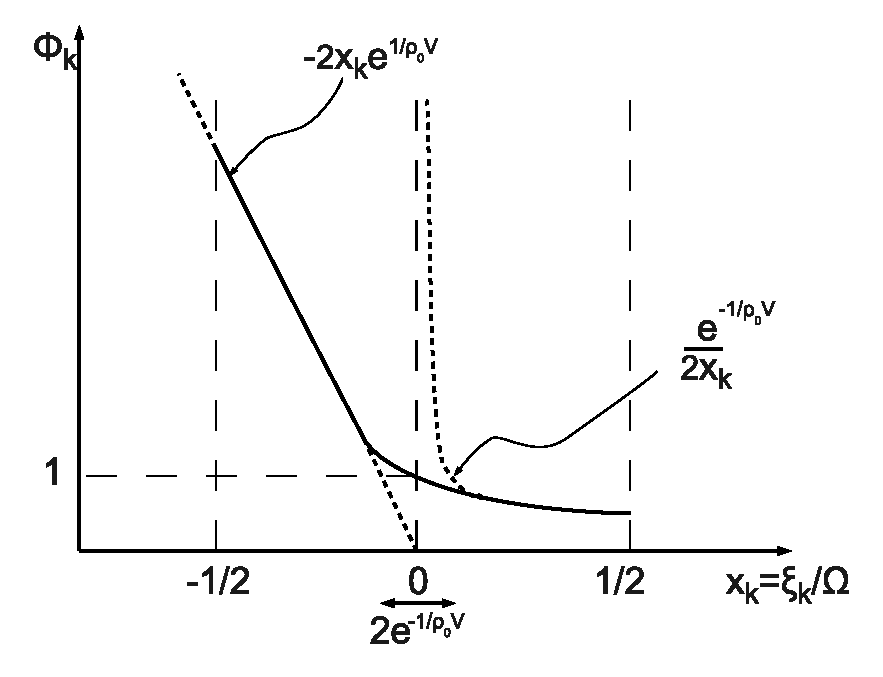
\includegraphics[width=0.5\textwidth]{BcsWF}
 \caption{BCS pair wave function\label{}}
 \end{figure}

In order to make clearer the relative weight of a given $\vk$ pair in this distribution, it is convenient to use the normalized BCS pair creation operator defined in Eq. (\ref{eq:c})
with $\langle{}F_0|CC^\dg|F_0\rangle=1$. The wave function then is $\varphi_\vk=\alpha^{-1}\phi_\vk$ with $\alpha\approx{}e^{1/\rho_0V}\sqrt{N_\Omega/6}$, as given in Eq.(\ref{eq:alpha}). This means that the number of pair having a sizable $\varphi_\vk$ are essentially between $\epsilon_{F_0}$ and  $\mu-\Delta/2$, this $\varphi_\vk$ value being of the order of 
\begin{equation}
 \varphi_1\approx\frac{1}{\sqrt{N_\Omega}}
\end{equation}
where $N_\Omega$ is the total number of pair feeling the potential.  This $\varphi_\vk$ distribution has a small tail of the order of 
\begin{equation}
  \varphi_2\approx\frac{e^{-1/\rho_0V}}{\sqrt{N_\Omega}}
\end{equation}
for pair with energy in the range $\pm\Delta/2$ around the chemical potential.  Pairs with higher energy are going to enter with a prefactor $\varphi_3^2\approx{}e^{-4/\rho_0V}/N_\Omega$. Consequently, its contribution in $e^{4/\rho_0V}$ is expected to be too small to produce relevant effect: most probably these high energy pairs play a negligible role in BCS superconductivity. 

The above analysis of the $\varphi_\vk$ wave function controlling the BCS composite boson operator $C^\dg$ leads us to think that Pauli blocking among these BCS pairs, which mainly affects the ones having a sizable $\varphi_\vk$, is going to have a dramatic effect for $N$ close to half filling, not to complete filling: this precisely is the value we want. 

Let us now study more in details how the $f_N$ factor of these $C^\dg$ pairs drops to zero in the $\Delta$ layer around the chemical potential $\mu$.  For that, we approximate the $\varphi_\vk$ distribution by a two-step distribution, with a first part equal to $\varphi_1$ extending between $\epsilon_{F_0}$ and $\mu-\Delta/2$ and a second part equal to $\varphi_2$ extending over $\mu\pm\Delta/2$. 


  The distribution probability of $\vk$ pairs in the BCS correlated pair is  given by 
\begin{equation}
p_\vk=\langle{}F_0|Ca^\dg_\vk{}a_\vk{}C^\dg|F_0\rangle=|\varphi_\vk|^2
\end{equation}

% Create the reference section using BibTeX:
%\bibliography{../citation}

\end{document}



